The analog to digital converter (ADC) is responsible for converting the analog voltage from the output of the Preamp, which is connected to the recording electrodes in the electrophysiology setup, into digital values at regular discrete time intervals.  According to the sampling theorem, the sampling frequency must be at least twice the highest frequency component of the analog signal to avoid loss of information in the analog to digital conversion~\cite{AlexanderSadiku2004}.  The Preamp has an output bandwidth of 20\unit{Hz} to 14.6\unit{kHz}~\cite{StahlMSEE}, which means that the minimum required sampling frequency, or Nyquist frequency, of the ADC must be $2\times14.6\unit{kHz}=29.2\unit{kHz}$~\cite{AlexanderSadiku2004}.  The AD7606 ADC from Analog Devices\textsuperscript{\textregistered} offers eight analog inputs with a selectable range of $\pm 10\unit{V}$ or $\pm 5\unit{V}$ with 16 bits of resolution that sample at up to $200\unit{kHz}$~\cite{AD7606ds}, and the AD7606 has been used previously in the Neurobiology Engineering Laboratory~\cite{BatzerCorsiCrampton}.  The AD7606 has an analog input filter with a corner frequency of $23\unit{kHz}$ at $\pm 10\unit{V}$ input range and $15\unit{kHz}$ at $\pm 5\unit{V}$ input range~\cite{BatzerCorsiCrampton}.

Figure~\ref{fig:ADC} shows the connections between the Xilinx\textsuperscript{\textregistered} XC3S500E FPGA on the RTSC board and the AD7606 on the Electrophysiology Interface board.  The FPGA GPIO pins connect to the digital interface of the AD7606 through the Hirose FX2 connectors and the signals are accessible on the 40-pin test header before going through a $0\unit{\Omega}$ resistor and finally connecting to the AD7606.  Signals not used in the FPGA configuration may have their $0\unit{\Omega}$ resistors unpopulated allowing the unused FPGA GPIO pins to be used for other purposes and accessed on the 40-pin test header.  There is a separate power supply pin, VDrive, on the AD7606 that drives the logic outputs and controls the thresholds of the logic inputs; VDrive should be powered to the same voltage as the GPIO supply of the FPGA~\cite{AD7606ds}.

\begin{figure}[H]
	\centering 
		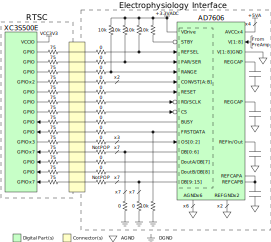
\includegraphics{./figures/AD} 
	\caption{FPGA connections to the ADC\label{fig:ADC}}
\end{figure}

The single-ended outputs of the Preamps are connected to the analog voltage inputs with all channel GND pins connected to AGND.  The main power supply is required to be $5\unit{V}$ $\pm 0.25\unit{V}$~\cite{AD7606ds}, so a $5\unit{V}$ regulator driven by +VA provides the AVCC power.  The Electrophysiology Interface board is setup for the AD7606 to use its internal voltage reference.  The AD7606 requires a $10\unit{\mu F}$ capacitor on the REFIn/Out pin for the operation of its internal voltage reference~\cite{AD7606ds}.  There are also a few capacitors needed for internal regulators and references; these pins have capacitors sized and placed according to the recommendation in the data sheet~\cite{AD7606ds}.  The details of the rest of the pin functions and connections are in Table~\ref{tab:AD7606Pins}.

\renewcommand{\arraystretch}{1.3}
%\begin{table}[H]
\begin{singlespace}
\centering 
\begin{longtable}[h]{|p{1.5in}|p{3.5in}|}
\multicolumn{2}{c}{{Table~\ref{tab:AD7606Pins}}} \\
\hline
Pin	& Function\\
\endhead
\multicolumn{2}{r}{\textit{Continued on next page}} \\
\endfoot
\endlastfoot
\hline
VDrive	& Digital supply voltage.  Should be the same voltage as FPGA GPIO\\
\hline
$\overline{\mathrm{STBY}}$	& Puts AD7606 into low power standby mode when LOW.  Tied to HIGH and not connected to FPGA\\
\hline
REFSEL	& Selects internal, HIGH, or external, LOW, voltage reference.  Pulled high through $10\unit{k\Omega}$ so $0\unit{\Omega}$ resistor may be unpopulated and FPGA GPIO used for other purpose\\
\hline
$\overline{\mathrm{PAR}}$/SER/BYTESEL	& Selects between serial, HIGH, or parallel, LOW, data interface.  If parallel interface is selected, this is read in conjunction with DB[15] to specify 8 or 16 bit parallel interface.  Pulled high through $10\unit{k\Omega}$ so $0\unit{\Omega}$ resistor may be unpopulated and FPGA GPIO used for other purpose\\
\hline
RANGE	& Sets analog input range at $\pm10\unit{V}$, HIGH, or $\pm10\unit{V}$, LOW.  Pulled high through $10\unit{k\Omega}$ so $0\unit{\Omega}$ resistor may be unpopulated and FPGA GPIO used for other purpose\\
\hline
CONVST[A:B]	& Conversion Start A initiates conversions on the lower half of the analog inputs (channels 1-4 for AD7606, 1-3 for AD7606-6, and 1-2 for AD7606-4) and Conversion Start B initiates conversions on the upper half of the analog inputs.  To sample on all channels simultaneously, switch both signals simultaneously.  These can be shorted if both are always going to be started simultaneously, saving a FPGA GPIO pin.\\
\hline
RESET	& Rising edge resets the AD7606.  The FPGA should issue a RESET pulse to the AD7606 upon power-up\\
\hline
$\overline{\mathrm{RD}}$/SCLK	& Parallel data read control or serial data clock input\\
\hline
$\overline{\mathrm{CS}}$	& Chip select input frames data transfer\\
\hline
BUSY	& Output rises after CONVST and falls after conversion is complete and data is ready to be clocked out\\
\hline
FRSTDATA	& Three-state output is high-impedance when $\overline{\mathrm{CS}}$ is HIGH, when $\overline{\mathrm{CS}}$ is LOW, FRSTDATA is LOW except during the $\overline{\mathrm{RD}}$ operation when channel 1 is on the parallel interface or when the 16 bits of channel 1 are being clocked out of DoutA on the serial interface (see~\cite{AD7606ds} for more information).  Pulled low through $10\unit{k\Omega}$ resistor to keep signal at known state when in three(tri)-state (high-impedance) mode.\\
\hline
OS[0:2]	& Over sampling mode select pins enables conversion a high sampling frequency and reading of the data at a lower frequency.  The AD7606 then applies a digital low-pass filter before making the data available on the parallel or serial interface.  Setting the mode pins to [0:0:0] disables the over sampling function.  Enabling the over sampling function affects effective input bandwidth.\\
\hline
DB[0:6]	& Three-state parallel digital input/output pins that should be tied to ground if serial data interface is used.  If using the AD7606 in serial mode $0\unit{\Omega}$ resistors to ground should be populated and $0\unit{\Omega}$ resistors to the FPGA should not be populated.  If using the AD7606 in parallel mode $0\unit{\Omega}$ resistors to ground should not be populated and $0\unit{\Omega}$ resistors to the FPGA should be populated.\\
\hline
DoutA/DB[7]	& If $\overline{\mathrm{PAR}}$/SER/BYTESEL is HIGH, it functions as DoutA and outputs serial conversion data. Channels 1 to 4 (1 to 3 for AD7606-6, 1 to 2 for AD7606-4) first appear on DoutA.  If $\overline{\mathrm{PAR}}$/SER/BYTESEL is LOW it's a three-state parallel digital input/output pin.\\
\hline
DoutB/DB[8]	& If $\overline{\mathrm{PAR}}$/SER/BYTESEL is HIGH, it functions as DoutB and outputs serial conversion data. Channels 1 to 4 (5 to 8 for AD7606-6, 3 to 4 for AD7606-4) first appear on DoutB. Can be used as a single Dout line, the channels appear in order 5-8 then 1-4.  If $\overline{\mathrm{PAR}}$/SER/BYTESEL is LOW it's a three-state parallel digital input/output pin.\\
\hline
DB[9:15]	& DB[15] is also an input pin and is read if $\overline{\mathrm{PAR}}$/SER/BYTESEL is LOW to select between 8 bit and 16 bit interface.  Three-state parallel digital input/output pins that should be tied to ground if serial data interface is used.  If using the AD7606 in serial mode $0\unit{\Omega}$ resistors to ground should be populated and $0\unit{\Omega}$ resistors to the FPGA should not be populated.  If using the AD7606 in parallel mode $0\unit{\Omega}$ resistors to ground should not be populated and $0\unit{\Omega}$ resistors to the FPGA should be populated.\\
\hline
REGCAP	& Decoupling capacitors for internal regulators.  Each pin should have a $1\unit{\mu F}$ capacitor as close to the pin as possible with the other end connected to ground.\\
\hline
REFIn/Out	& Voltage reference in or out.  The pin should have a $10\unit{\mu F}$ capacitor as close to the pin as possible with the other end connected to ground.\\
\hline
REFCAP[A:B]	& Reference buffer output force/sense pins.  These pins should be tied together and have a $10\unit{\mu F}$ low ESR, ceramic capacitor as close to the pin as possible with the other end connected to ground.\\
\hline

\caption{Notes on AD7606 ADC pin connections and functions with information from~\cite{AD7606ds}\label{tab:AD7606Pins} }
\end{longtable}


\end{singlespace}
%\end{table}
\renewcommand{\arraystretch}{1.0}

